\section{April Tag Modifications}
\label{section:apriltag_modifications}

April Tag~\cite{apriltag_paper}\cite{apriltag2_paper}\cite{apriltag3_paper} is a popular fiducial marker formed by a series of black and white squares.
Several marker families are available, each with its own layout, as shown in Figure~\ref{figure:apriltags}.
The essential parts of the marker include a square border of black squares with a white border on the inside.
Other square sections can either be ``data bits'' which contribute to the ID of the marker,
or they can be unused and either not contribute to the marker definition at all, or provide a place for embedding another tag.

\begin{figure}
    \centering
    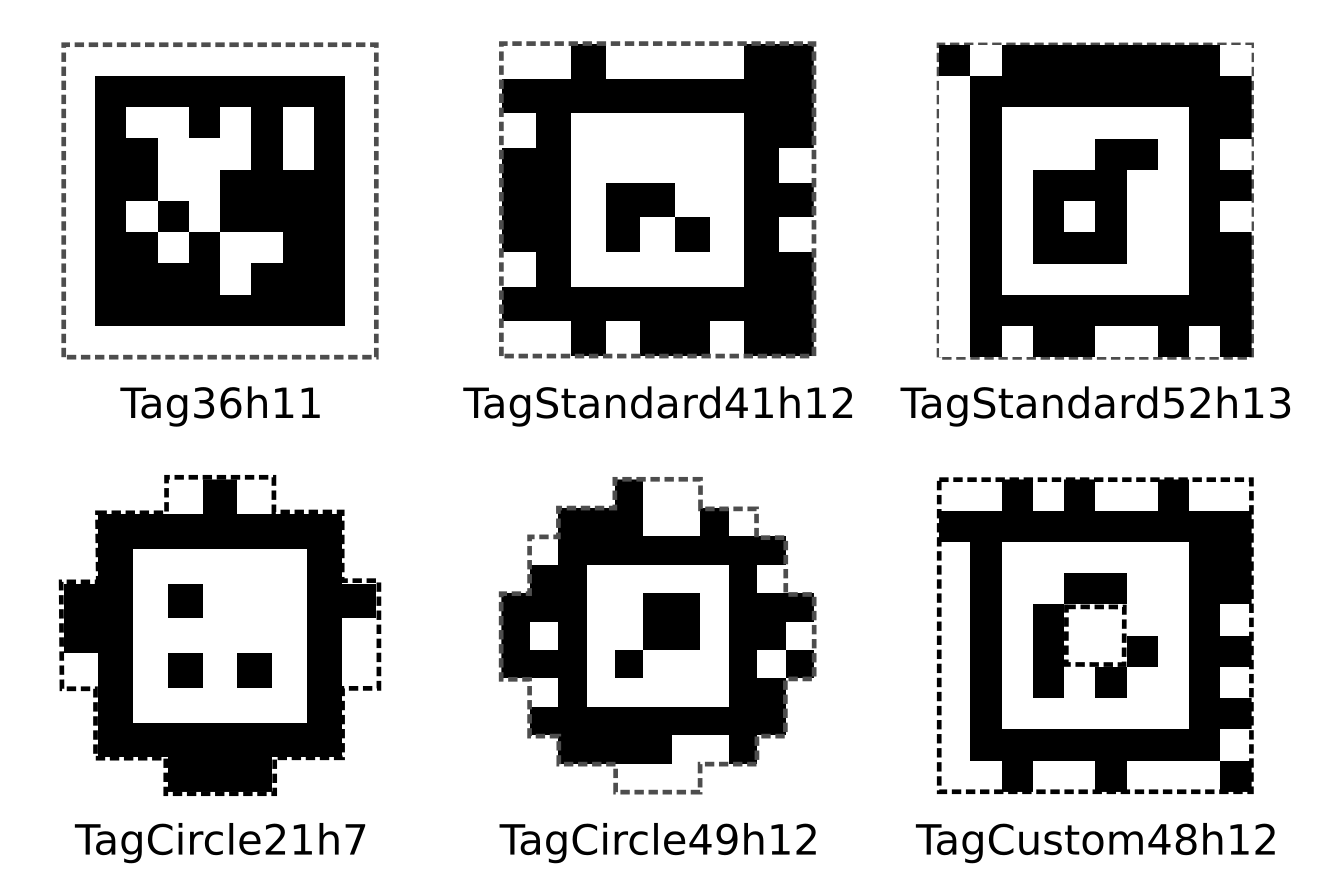
\includegraphics[width=0.75\textwidth]{images/apriltags}
    \caption{Several available April Tag families (from the paper Flexible Layouts for Fiducial Tags~\cite{apriltag3_paper})}
    \label{figure:apriltags}
\end{figure}

April Tag markers, in contrast to WhyCode markers, cannot be recognized independently of their ID.
A benefit of this is that each marker can be assigned its own size before runtime,
so many markers of different sizes and IDs can be used simultaneously.
Figure~\ref{figure:apriltags}f shows the family April Tag 48h12, which has 48 ID bits,
and where each valid ID has a hamming distance of at least 12 from the others.
When the April Tag family is generated, all arrangements of black and white squares
that fit the requirements of the family definition (as well as isomorphic versions)
are put into a hash table that is used to determine the validity of detected tags at runtime.

The 48h12 family has 4 undefined bits in its center, where another marker in the same family can be placed.
This marker embedding is crucial for drone landing because it allows the drone to have
reliable pose estimation throughout the entire landing.
For example, if a landing pad uses a single marker that is recognizable from far away,
it is likely that the marker will not be visible during the last stages of landing
where the marker may eclipse the camera's field of view.
Non-embedded markers of different sizes can be placed on a landing pad in non-intersecting positions,
but this implies more complications in tracking the markers during landing.
Embedding concentric markers in one another and marking them as a tag bundle reduces the complexity
regarding coordinate system transforms and tracking.
The 48h12 family is therefore a natural candidate for marking landing pads.

\subsection{Re-testing in Simulation with April Tag 48h12}

After moving away from the WhyCode system for the purpose of autonomous landing, I re-implemented the method
from the thesis to use only embedded 48h12 April Tags and re-tested successfully in simulation.
The re-implementation involved adding to the April Tag ROS code with special focus on
tag bundles,
marker tracking,
and coordinate system transforms.
The landing pads are defined as concentric, co-planar tag bundles with the same yaw orientation
that take the position and orientation of their largest detected marker,
expose their pixel centers $u,v$ (for PID tracking),
and calculate their camera translation (position rotated by the inverse of their orientation)
before exposure to other ROS nodes through messages.
The code is available at its Github repository ~\cite{edited_apriltag}.
The marker bundle forming the landing pad is shown in Figure \ref{figure:landing_pad_apriltag_48h12_3_2_1_0}.

The re-implementation was successful in simulation\footnote{Video from testing this method in simulation with April Tag 48h12 embedded markers can be found here: \url{https://vimeo.com/manage/videos/526223833}}, as shown by the landing trajectories in Figure~\ref{figure:apriltag48h12_landings}.
Additionally, the marker bundle tracking allowed for robust, uninterrupted tracking during landing, as shown by Figure~\ref{figure:apriltag48h12_landings_tracking}.

\begin{figure}
    \centering
    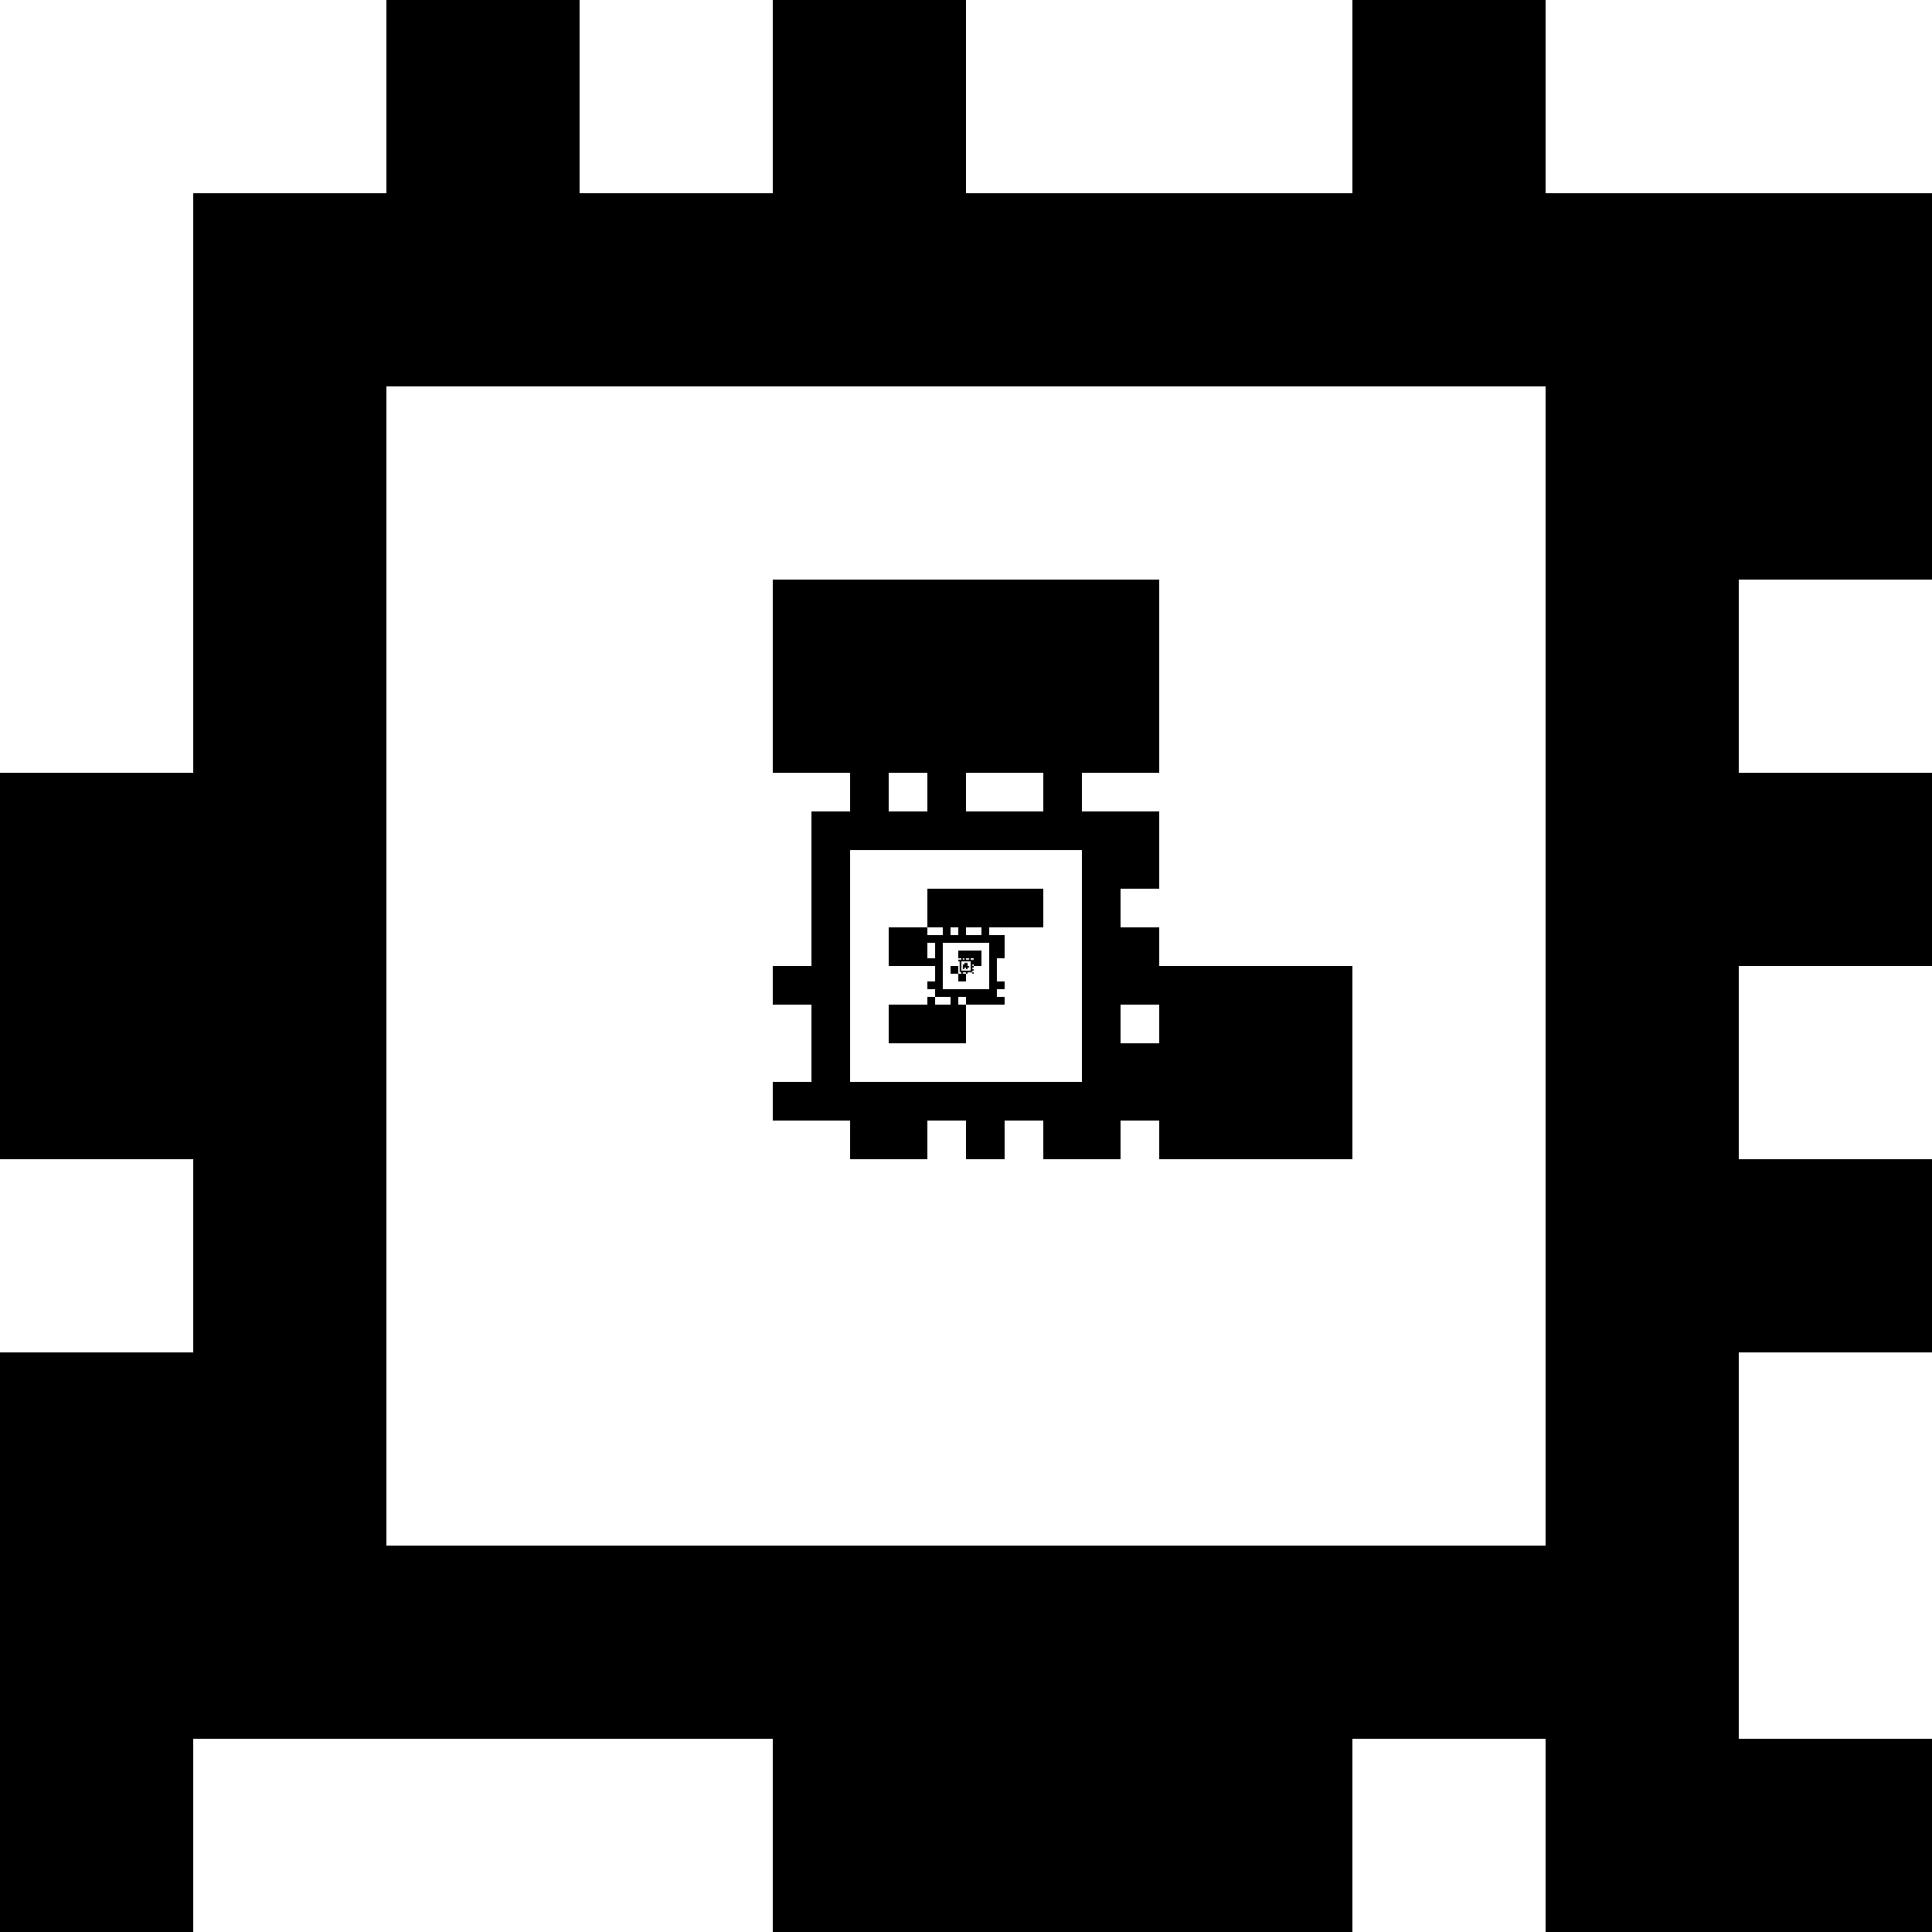
\includegraphics[width=0.5\textwidth]{images/landing_pad_apriltag_48h12_3_2_1_0}
    \caption{The landing pad for the given tests, with 48h12 IDs 3, 2, 1, and 0 in order of decreasing size.}
    \label{figure:landing_pad_apriltag_48h12_3_2_1_0}
\end{figure}

\begin{figure}
    \center
    \begin{subfigure}[b]{0.49\textwidth}
         \centering
         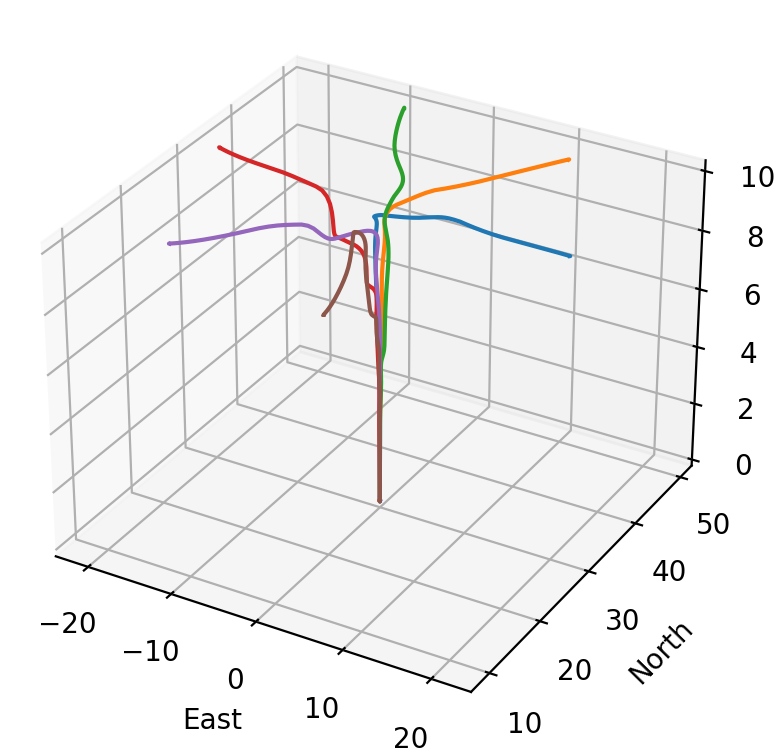
\includegraphics[width=\textwidth]{images/landing_trajectories}
    \end{subfigure}
    \hfill
    \begin{subfigure}[b]{0.49\textwidth}
         \centering
         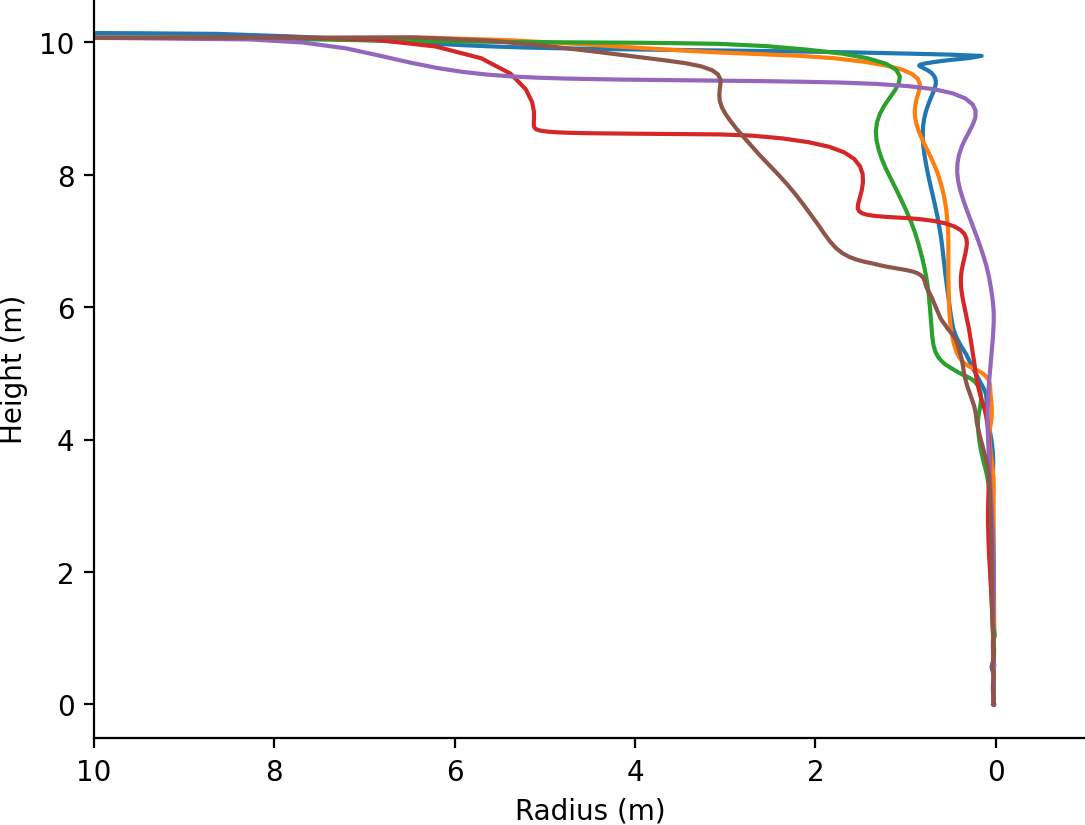
\includegraphics[width=\textwidth]{images/radius_vs_height}
    \end{subfigure}
    \caption{Left: landing trajectories for a series of simulated landings, centered around the landing pad. Right: the horizontal distance of the drone from the landing pad versus its height during landing. Both: these landings are executed by the code from the original thesis, using ArduPilot.}
    \label{figure:apriltag48h12_landings}
\end{figure}

\begin{figure}
    \center
    \begin{subfigure}[b]{0.49\textwidth}
         \centering
         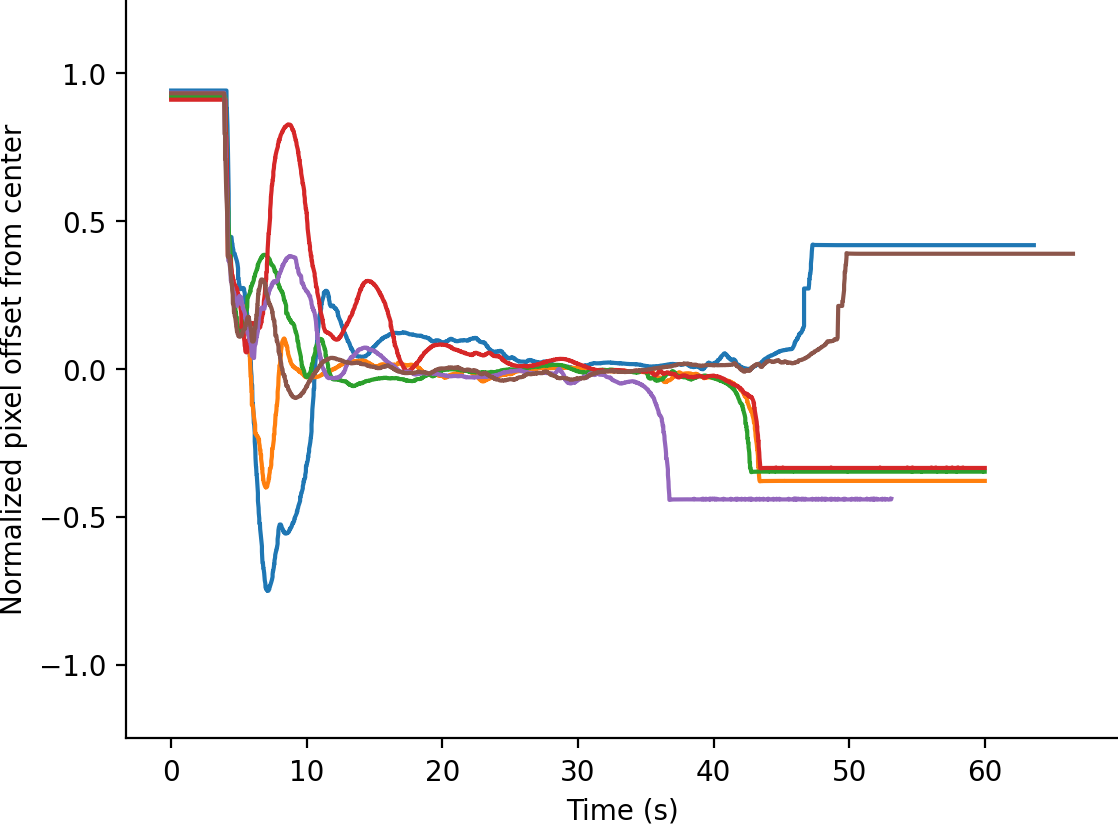
\includegraphics[width=\textwidth]{images/visual_center_x}
    \end{subfigure}
    \hfill
    \begin{subfigure}[b]{0.49\textwidth}
         \centering
         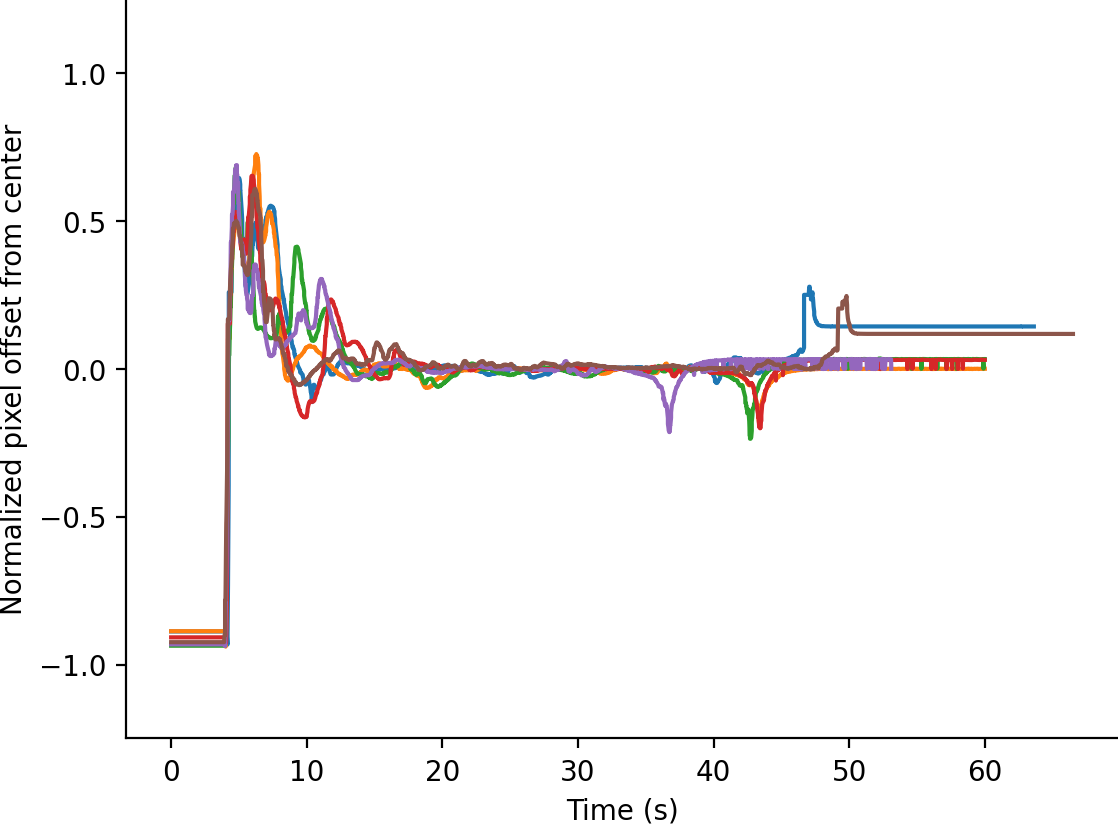
\includegraphics[width=\textwidth]{images/visual_center_y}
    \end{subfigure}
    \caption{Pixel positions of the landing pad marker bundle during the landings depicted in Figure~\ref{figure:apriltag48h12_landings}.}
    \label{figure:apriltag48h12_landings_tracking}
\end{figure}

\subsection{Testing on Physical Hardware, and the creation of April Tag 24h10}

A fundamental limitation of simulation in general is that it does not allow one to test all aspects of a given system.
In contrast to simulated experiments on a desktop, which could easily run April Tag 48h12 at $\geq30$ Hz,
initial experiments on a Raspberry Pi 3 showed that
the system was only able to analyze 640x480 pixel images at a rate of 1.5Hz,
which is not sufficient for a precision landing.
Additionally, the 42211 markers of the 48h12 family create a huge (> 1 GB) hash table
on the Raspberry Pi, needlessly hogging valuable memory.
However, no other default family of April Tags allows for marker embedding.
This necessitated a new marker family that both allows for marker embedding and has sufficiently fast runtime performance
on embedded hardware such as a Raspberry Pi 3 - April Tag 24h10.
This family attemps to minimize the size of the markers,
maximize the number of marker IDs in the family,
and maintain the ability to embed markers.
The definition is shown in Table \ref{table:apriltag_24h10_definition}, and the set of valid markers in Figure~\ref{figure:apriltag24h10}.

\begin{table}[]
    \centering
\begin{tabular}{
>{\columncolor[HTML]{C0C0C0}}c
>{\columncolor[HTML]{FFFFFF}}c ccc
>{\columncolor[HTML]{FFFFFF}}c
>{\columncolor[HTML]{C0C0C0}}c }
{\color[HTML]{333333} d} & \cellcolor[HTML]{C0C0C0}{\color[HTML]{333333} d} & \cellcolor[HTML]{C0C0C0}{\color[HTML]{333333} d} & \cellcolor[HTML]{C0C0C0}{\color[HTML]{333333} d} & \cellcolor[HTML]{C0C0C0}{\color[HTML]{333333} d} & \cellcolor[HTML]{C0C0C0}{\color[HTML]{333333} d} & {\color[HTML]{333333} d} \\
{\color[HTML]{333333} d} & {\color[HTML]{333333} w}                         & \cellcolor[HTML]{FFFFFF}{\color[HTML]{333333} w} & \cellcolor[HTML]{FFFFFF}{\color[HTML]{333333} w} & \cellcolor[HTML]{FFFFFF}{\color[HTML]{333333} w} & {\color[HTML]{333333} w}                         & {\color[HTML]{333333} d} \\
{\color[HTML]{333333} d} & {\color[HTML]{333333} w}                         & \cellcolor[HTML]{333333}{\color[HTML]{FFFFFF} b} & \cellcolor[HTML]{333333}{\color[HTML]{FFFFFF} b} & \cellcolor[HTML]{333333}{\color[HTML]{FFFFFF} b} & {\color[HTML]{333333} w}                         & {\color[HTML]{333333} d} \\
{\color[HTML]{333333} d} & {\color[HTML]{333333} w}                         & \cellcolor[HTML]{333333}{\color[HTML]{FFFFFF} b} & \cellcolor[HTML]{3166FF}{\color[HTML]{FFFFFF} x} & \cellcolor[HTML]{333333}{\color[HTML]{FFFFFF} b} & {\color[HTML]{333333} w}                         & {\color[HTML]{333333} d} \\
{\color[HTML]{333333} d} & {\color[HTML]{333333} w}                         & \cellcolor[HTML]{333333}{\color[HTML]{FFFFFF} b} & \cellcolor[HTML]{333333}{\color[HTML]{FFFFFF} b} & \cellcolor[HTML]{333333}{\color[HTML]{FFFFFF} b} & {\color[HTML]{333333} w}                         & {\color[HTML]{333333} d} \\
{\color[HTML]{333333} d} & {\color[HTML]{333333} w}                         & \cellcolor[HTML]{FFFFFF}{\color[HTML]{333333} w} & \cellcolor[HTML]{FFFFFF}{\color[HTML]{333333} w} & \cellcolor[HTML]{FFFFFF}{\color[HTML]{333333} w} & {\color[HTML]{333333} w}                         & {\color[HTML]{333333} d} \\
{\color[HTML]{333333} d} & \cellcolor[HTML]{C0C0C0}{\color[HTML]{333333} d} & \cellcolor[HTML]{C0C0C0}{\color[HTML]{333333} d} & \cellcolor[HTML]{C0C0C0}{\color[HTML]{333333} d} & \cellcolor[HTML]{C0C0C0}{\color[HTML]{333333} d} & \cellcolor[HTML]{C0C0C0}{\color[HTML]{333333} d} & {\color[HTML]{333333} d}
\end{tabular}
    \vspace*{0.5cm}
    \caption{Definition for the April Tag 24h10 family. Each square is marked by a letter representing its function.
    Data squares are marked as `d,' white squares as `w,' black sqares as `b,' and unused squares as `x.'}
    \label{table:apriltag_24h10_definition}
\end{table}

\begin{figure}
    \centering
    
\includegraphics[width=\textwidth]{tag24h10_mosaic_grey_background}
    \caption{The set of markers in the April Tag 24h10 family. The grey squares are not part of the marker definitions.}
    \label{figure:apriltag24h10}
\end{figure}

\subsection{Testing with PX4's Precision Land}

April Tag is subject to orientation ambiguity, similar to the WhyCon/WhyCode markers mentioned in Section \ref{section:whycode_modifications}.
When conducting an autonomous landing via a series of position setpoints, such as in the original thesis~\cite{joshua_master_thesis},
the orientation ambiguity is not prohibitively destructive - essentially because the orientation is correct ``most of the time.''
However, when using a method such as PX4's precision land function, a single orientation flip can make the landing fail.
This is because the method involves approaching the landing pad horizontally first (facing the landing pad directly),
and then descending vertically once the drone is adequately close.
The algorithm assumes it has reached or surpassed the landing pad location once it gets a single erroneous pose estimate for the landing pad.

One way around this issue is to simply filter the raw position estimate data with a Kalman filter, as shown in Figure \ref{figure:filtered_unfiltered_apriltag_24h10}.
The red data points represent the raw data, and the blue, continuous line represents the filtered position estimate
that is passed to the PX4 flight software.
Since the drone approaches the landing pad head-on, the ``north'' component of the landing pad's position is typically
the largest.
(This is just to say that the landing pad is in front of the drone, not to the side.)
Thus, filtering is most important in the case of the north component.
If the orientation flips (thereby causing a sign flip in the position),
the drone will think that it has already passed the landing pad, and will attempt to land wherever it happens to be
when the flip happens.
The particularly dangerous data points are therefore the negative outliers in the early stages of the landing.
Filtering is useful on the east component to reduce noise.
Filtering is not essential on the up component because orientation flipping does not change the perceived height.
Variation in the up component is simply considered noise.
In spite of the fluctuating raw and filtered values, the position estimate data can be used for precision landing,
as demonstrated in Figure \ref{figure:px4_precland_trajectories} which shows the horizontal distance from the landing pad versus altitude for multiple such landings.

\begin{figure}
    \center
    \begin{subfigure}[b]{0.49\textwidth}
         \centering
         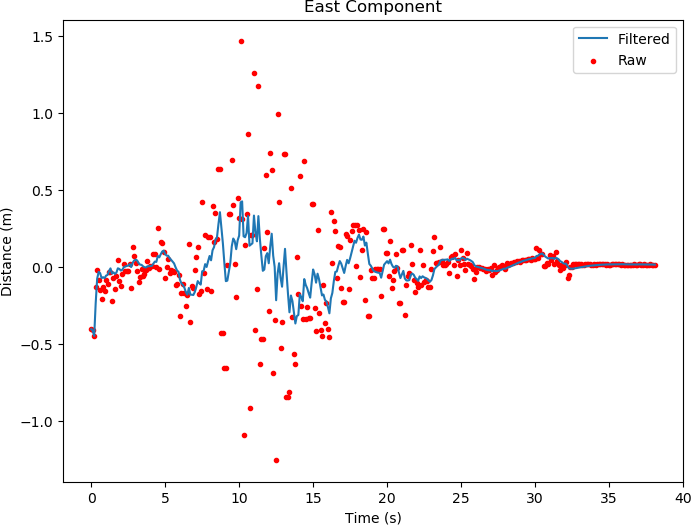
\includegraphics[width=\textwidth]{images/landing_apriltag24h10_east}
    \end{subfigure}
    \hfill
    \begin{subfigure}[b]{0.49\textwidth}
         \centering
         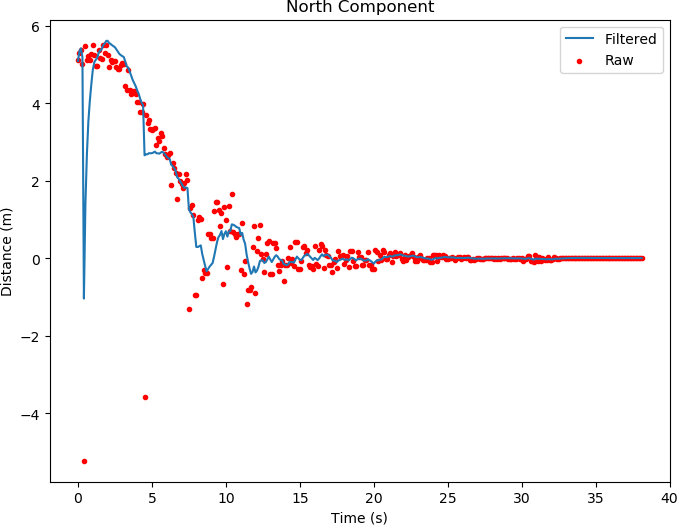
\includegraphics[width=\textwidth]{images/landing_apriltag24h10_north}
    \end{subfigure}

    \begin{subfigure}[b]{0.49\textwidth}
         \centering
         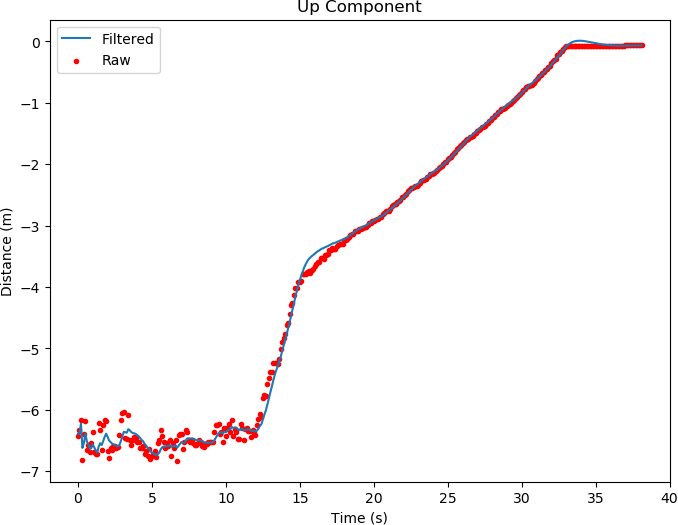
\includegraphics[width=\textwidth]{images/landing_apriltag24h10_up}
    \end{subfigure}
    \caption{Unfiltered and filtered estimates of the landing pad's position during landing.}
    \label{figure:filtered_unfiltered_apriltag_24h10}
\end{figure}

\begin{figure}
    \centering
    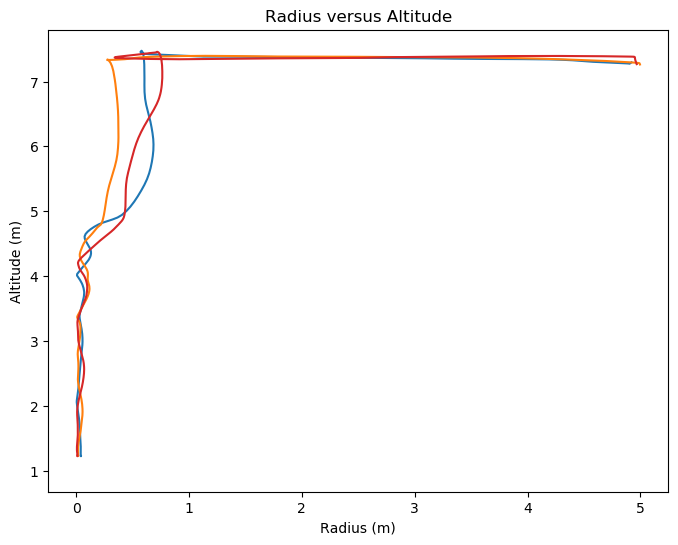
\includegraphics[width=0.49\textwidth]{px4_precland_trajectories}
    \caption{Horizontal distance from the landing pad versus altitude for 3 PX4 precision landings using the filtered April Tag 24h10 system.
    This graph should be read as if the drone is approaching from the right and moving left.}
    \label{figure:px4_precland_trajectories}
\end{figure}

\subsection{Conclusion}

Both the April Tag and WhyCon/WhyCode systems suffer from fundamental issues of orientation ambiguity.
April Tag's more intricate structure makes its perception of orientation more robust than that of WhyCon/WhyCode,
but it still does not eliminate the ambiguity entirely, and we can see the destructive consequences of this if the
orientation is used in other calculations.
Still, simple Kalman filtering can mitigate the issue enough that the system can be used for precision landing.
Furthermore, the flexible layout of April Tag makes it a better choice for precision landing.
The ability to embed concentric markers within each other is critical to maintaining a continuous view of the landing pad
from both near and far,
and the ability to change the number and layout of data bits allows users to adjust the markers according to their computational constraints.